\documentclass{article}

\usepackage{hyperref}
\usepackage{comment}
\usepackage{enumerate}
\usepackage{multirow}
\usepackage{makecell}
\usepackage{geometry}
\usepackage[shortlabels]{enumitem}
\usepackage{tabularx,ragged2e,booktabs,caption}
\usepackage{longtable}
\usepackage{float}
\usepackage{graphicx}
\usepackage{pdflscape}


\hypersetup{
    colorlinks=true,       % false: boxed links; true: colored links
    linkcolor=red,          % color of internal links (change box color with linkbordercolor)
    citecolor=green,        % color of links to bibliography
    filecolor=magenta,      % color of file links
    urlcolor=cyan           % color of external links
}

\title{Hazard Analysis\\\progname}

\author{\authname}

\date{}

%% Comments

\usepackage{color}

\newif\ifcomments\commentstrue %displays comments
%\newif\ifcomments\commentsfalse %so that comments do not display

\ifcomments
\newcommand{\authornote}[3]{\textcolor{#1}{[#3 ---#2]}}
\newcommand{\todo}[1]{\textcolor{red}{[TODO: #1]}}
\else
\newcommand{\authornote}[3]{}
\newcommand{\todo}[1]{}
\fi

\newcommand{\wss}[1]{\authornote{magenta}{SS}{#1}} 
\newcommand{\plt}[1]{\authornote{cyan}{TPLT}{#1}} %For explanation of the template
\newcommand{\an}[1]{\authornote{cyan}{Author}{#1}}

%% Common Parts

\newcommand{\progname}{SFWRENG 4G06 - Capstone Design Process}
\newcommand{\authname}{\textbf{Team 17, DomainX} \\
\\ Awurama Nyarko
\\ Haniye Hamidizadeh
\\ Fei Xie
\\ Ghena Hatoum             
}
\usepackage{hyperref}
    \hypersetup{colorlinks=true, linkcolor=blue, citecolor=blue, filecolor=blue,
                urlcolor=blue, unicode=false}
    \urlstyle{same}
                                


\begin{document}

\maketitle
\thispagestyle{empty}

\begin{table}[hp]
\caption{Revision History} \label{TblRevisionHistory}
\begin{tabularx}{\textwidth}{llX}
\toprule
\textbf{Date} & \textbf{Developer(s)} & \textbf{Change}\\
\midrule
October 6, 2025  & Whole team & Initial v0 Draft\\
October 29, 2025 & Fei & Update from TA feedback\\
\bottomrule
\end{tabularx}
\end{table}

~\newpage
\thispagestyle{empty}

\tableofcontents

~\newpage

\pagenumbering{arabic}

\section{Introduction}


This Hazard Analysis identifies and evaluates potential risks associated with
the DomainX Assessment Tool, a web-based application that
automates evidence collection, data storage, and visualization for assessing
open-source neural network libraries. 

In this context, a hazard is defined as any condition, event, or design
decision that could lead to loss of data integrity, software malfunction,
degraded performance, or failure to meet stakeholder requirements.

The tool integrates \href{https://react.dev/}{React} (frontend), \href{https://www.djangoproject.com/}{Django} (backend), and \href{https://www.mysql.com/}{MySQL}
(relational database), and public Application Programming Interfaces (APIs), such as the
GitHub API, to support automated data gathering, Analytic Hierarchy Process
(AHP)--based ranking, and visualization of software-quality metrics.

Because the system involves data integration, user interaction, and deployment
on university infrastructure, it faces technical and operational hazards, such as integration errors, API limits, and performance bottlenecks. This
document identifies such risks early in the lifecycle to protect software
reliability, data integrity, and user experience.

\section{Scope and Purpose of Hazard Analysis}

The purpose of this hazard analysis is to systematically identify potential
risks that could impact the reliability, usability, and delivery of the NNL
Assessment Tool.

Although the tool is non-safety-critical, losses could still occur through:

\begin{itemize}
    \item Data loss or corruption, affecting research integrity.
    \item System downtime, delaying project milestones or access for the research team.
    \item Inaccurate visualizations or metrics, leading to incorrect conclusions in research outputs.
    \item Security breaches, risking exposure of user accounts or evaluation data.
    \item Integration failures, which could prevent essential automation and data collection.
\end{itemize}

These losses would directly reduce the tool’s credibility, hinder academic
progress, and compromise user trust.

The analysis focuses on identifying, classifying, and mitigating these hazards
early to minimize risks and ensure project success.

\section{System Boundaries and Components}

The following explain the System Components:
\begin{enumerate}[label=C\arabic*.]
  \item Admin UI: Handles invitation, domain creation, and user management views.
  \item Researcher UI: Handles data input, update, and visualization controls.
  \item User Management: Handles logic for invite/sign-up, login, roles, and password reset.
  \item Domain Data Service: Handles read and write operations for Domains, Libraries, and Metrics.
  \item AHP Ranking: Handles the AHP calculation.
  \item Visualization: Handles graph generation.
  \item Export: Handles data downloads (JSON/Excel).
  \item Security: Handles Access Control, validation, encrypt password, and manages audit trails.
  \item Persistence: Handles storage and retrieval for all data entities.
  \item System Database: The underlying data store.
\end{enumerate}

\begin{figure}[H]
    \centering
    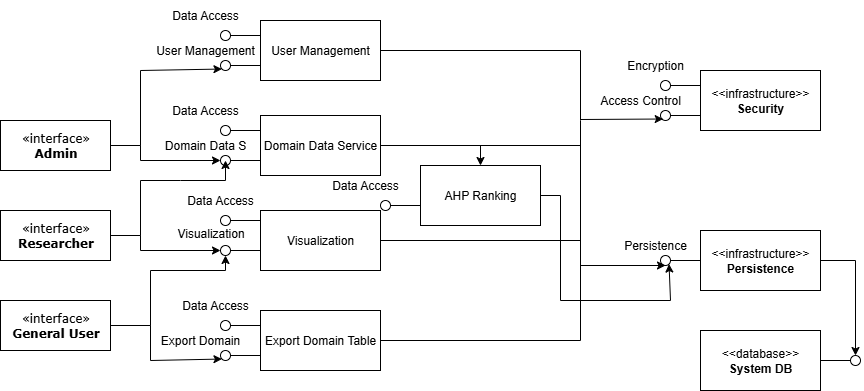
\includegraphics[scale=0.5] {images/component.png}
    \caption{System Components Table}
\end{figure}

\section{Critical Assumptions}

The following assumptions support hazard identification and mitigation:

\begin{itemize}
    \item \textbf{Access to Public APIs:} It is assumed that GitHub API and other
    data sources will remain stable; however, if access limits or outages occur,
    fallback mechanisms (e.g., cached data, manual upload) will be implemented.
    
    \item \textbf{McMaster Infrastructure Availability:} University servers will
    host the tool; if unavailable, contingency hosting (local or alternative
    cloud) will be explored.
    
    \item \textbf{Stable Development Team:} All members remain active; if a
    member becomes unavailable, roles and documentation ensure continuity.
    
    \item \textbf{Non-Safety-Critical Context:} Hazards relate to data and
    usability, not physical harm, but errors could still cause loss of
    credibility or project delays.
    
    \item \textbf{Defined Scope and Requirements:} Requirements remain stable;
    changes will trigger re-assessment of risks.
    
    \item \textbf{Version Control and Standards:} Git workflow reduces
    integration errors, though merge conflicts remain possible; peer reviews
    mitigate these.
    
    \item \textbf{User Feedback Availability:} Testing feedback will be
    accessible; if delayed, internal testing will substitute temporarily.
\end{itemize}

\section{Failure Mode and Effect Analysis}
This contains the Failure Mode and Effect Analysis table below and is a breakdown of the hazards that could occur within the system, along with recommended actions to mitigate them.
\newgeometry{margin=0.5in}
\begin{landscape}
  \begin{longtable}{|p{2cm}|p{4cm}|p{4cm}|p{4cm}|p{4cm}|p{2cm}|p{2cm}|}
  \caption{Failure Mode and Effect Analysis} \label{FMEA}\\
  \hline
   Component & Failure Modes & Effects of Failure & Causes of Failure & Recommended Action & SR & Ref.  \\ 
  \hline
  \endfirsthead
  \multicolumn{7}{r}{Table \thetable\ Continued from previous page}\\ 
  \hline
   Design Function & Failure Modes & Effects of Failure & Causes of Failure & Recommended Action & SR & Ref.  \\ 
  \hline
  \endhead
  \multicolumn{7}{r}{{Continued on next page}}\\
  \endfoot
  \multicolumn{7}{r}{{Concluded}}\\
  \endlastfoot
  \multirow{7}{*}{User account} & 
  \begin{enumerate}[leftmargin=*]
    \item User can't login/sign-up.
    \item Cannot set correct role for user.
    \item User account information is leaked.
  \end{enumerate} & 
  \begin{enumerate}[leftmargin=*]
    \item User cannot access their work.
    \item Refer to H1-1.
    \item User credentials are exposed, exposing them to cyber attack or data scrapers.
  \end{enumerate} &
  \begin{enumerate}[leftmargin=*]
    \item
    \begin{enumerate}
        \item[a)] Integration with database failure.
        \item[b)] User entered incorrect credentials.
    \end{enumerate}
    \item Refer to H1-1.a.
    \item Weak access controls, lack of encryption, or insecure credentials.
  \end{enumerate} &
  \begin{enumerate}[leftmargin=*]
    \item 
    \begin{enumerate}
        \item[a)] Implement automated daily system integration testing.
        \item[b)] Provide user feedback during user actions.
        \item[c)] Provide option for resetting credentials.
    \end{enumerate}
    \item Refer to H1-1.a, H1-1.b, H1-1.c.
    \item 
    \begin{enumerate}
        \item[a)] Implement authentication techniques and follow industry best practices for security.
        \item[b)] Validate inputs for common security vulnerabilities, such as SQL injections.
    \end{enumerate}
  \end{enumerate} &
  \begin{enumerate}[leftmargin=*]
    \item SR-AC5, MS-MR4, PR-RFT3.
    \item SR-AC2, SR-AC4.
    \item SR-P1, SR-P2, SR-IM1, SR-IM2, PR-SC1, PR-SC2.
  \end{enumerate} &
  \begin{enumerate}[leftmargin=*]
    \item H1-1
    \item H1-2
    \item H1-3
  \end{enumerate} \\
  \hline
  \multirow{7}{*}{\makecell{Domain\\Creation}} & 
  \begin{enumerate}[leftmargin=*]
      \item Cannot create new domains
      \item Cannot edit existing domain
  \end{enumerate} & 
  \begin{enumerate}[leftmargin=*]
    \item
    \begin{enumerate}
        \item[a)] User cannot continue their work on the domain
        \item[b)] User will be delayed when writing their analysis
    \end{enumerate}
    \item Refer to H2-1.a, H2-1.b.
  \end{enumerate} &
  \begin{enumerate}[leftmargin=*]
    \item  Refer to H1-1.a
    \begin{enumerate}
        \item[a)] User has incorrect access control level
        \item[b)] Database failure, all data on the database removed
    \end{enumerate}
    \item Refer to H1-1.a, H2-1.a, H2-1.b.
  \end{enumerate} &
  \begin{enumerate}[leftmargin=*]
       \item Refer to H1-1.a, H1-1.b.
       \begin{enumerate}
        \item[a)] Implement backup databases and backup protocols
    \end{enumerate}
       \item  Refer to H1-1.a, H1-1.b.
  \end{enumerate} &
  \begin{enumerate}[leftmargin=*]
       \item SR-AC3, SR-AC4, PR-RFT2
       \item SR-AC2, SR-AC3, SR-AC4
  \end{enumerate} &
  \begin{enumerate}[leftmargin=*]
       \item H2-1
       \item H2-2
  \end{enumerate} \\
  \hline
  \multirow{7}{*}{\makecell{Adding Data\\to a Domain}} & 
  \begin{enumerate}[leftmargin=*]
      \item User cannot add new data point
      \item User cannot update existing data point
      \item Automated process overwriting user data unknowingly
      \item Automated data input failure
  \end{enumerate} & 
  \begin{enumerate}[leftmargin=*]
      \item Refer to H2-1.a, H2-1.b.
      \item Refer to H2-1.a, H2-1.b.
      \item Refer to H2-1.a, H2-1.b 
      \begin{enumerate}
        \item[a)] Loss of user trust towards the tool
    \end{enumerate}
      \item Refer to H2-1.a, H2-1.b,
      \begin{enumerate}
        \item[a)] User has to manually input data, reducing usefulness of the tool
    \end{enumerate}
  \end{enumerate} &
  \begin{enumerate}[leftmargin=*]
       \item Refer to H1-1.a
       \begin{enumerate}
            \item[a)] Network issues
            \item[b)] Save conflict occurring when multiple users are trying to edit the same data point
        \end{enumerate}
       \item Refer to H1-1.a, H3-1.a, H3-1.b
       \item 
       \begin{enumerate}
            \item[a)] Lack of user training on how automated data points work
            \item[b)] Inadequate user feedback user during system processes
        \end{enumerate}
       \item Refer to H3-1.a.
       \begin{enumerate}
            \item[a)] Integration issues with external systems
        \end{enumerate}
  \end{enumerate} &
  \begin{enumerate}[leftmargin=*]
    \item Refer to H1-1.a, H1-1.b.
    \begin{enumerate}
        \item[a)] Explicit visual block on data points that other users are editing
    \end{enumerate}
    \item Refer to H1-1.a, H1-1.b, H3-1.a.
    \item Refer to H1-1.a, H1-1.b
    \begin{enumerate}
        \item[a)] Provide explicit user controls for manual inputs
        \item[b)] Provide training on key features to user
        \item[c)] Implement confirmation system for automated sections
    \end{enumerate}
    \item Refer to H1-1.a, H1-1.b, H3-1.a.
  \end{enumerate} &
  \begin{enumerate}[leftmargin=*]
    \item SR-INT1, SR-INT2, SR-INT3, PR-RFT2.
    \item SR-INT1, SR-INT2, SR-INT3, PR-RFT2.
    \item SR-INT4, SR-INT5, PR-RFT2.
    \item SR-INT1, SR-AC6, SR-IM3, SR-IM4, PR-RFT2.

  \end{enumerate} &
  \begin{enumerate}[leftmargin=*]
    \item H3-1
    \item H3-2
    \item H3-3
    \item H3-4
  \end{enumerate} \\
  \hline
  \multirow{7}{*}{\makecell{Data\\Visualization}} & 
  \begin{enumerate}[leftmargin=*]
      \item Visualization method does not match data points
  \end{enumerate} & 
  \begin{enumerate}[leftmargin=*]
      \item Refer to H2-1.b, H3-3.a.
  \end{enumerate} &
  \begin{enumerate}[leftmargin=*]
    \item Refer to H1-1.a
    \begin{enumerate}
        \item[a)] External system used for visualization not properly configured/working
        \item[b)] Another user is editing the data points while current user is trying to visualize
    \end{enumerate}
  \end{enumerate} &
  \begin{enumerate}[leftmargin=*]
    \item Refer to H1-1.A
    \begin{enumerate}
        \item[a)] Require user to lock the domain when editing, with visualization functionality being available only on unlocked domains.
    \end{enumerate}
  \end{enumerate} &
  \begin{enumerate}[leftmargin=*]
       \item SR-INT6
  \end{enumerate} &
  \begin{enumerate}[leftmargin=*]
       \item H4-1
  \end{enumerate} \\
  \hline
  \multirow{7}{*}{\makecell{Download\\Data}} & 
  \begin{enumerate}[leftmargin=*]
    \item User unable to download the data/visuals of a domain
    \item Downloaded data/visuals of a domain are corrupted and unusable
  \end{enumerate} & 
  \begin{enumerate}[leftmargin=*]
      \item Refer to H2-1.b.
      \item Refer to H2-1.b, H3-3.a.
  \end{enumerate} &
  \begin{enumerate}[leftmargin=*]
    \item Refer to H1-1.a, H2.1.a, H3-1.a, H4-1.a.
    \item Refer to H1-1.a, H3-1.a, H4-1.a.
  \end{enumerate} &
  \begin{enumerate}[leftmargin=*]
       \item Refer to H1-1.a, H1-1.b.
       \begin{enumerate}
        \item[a)] Provide multiple methods for downloading or sharing
    \end{enumerate}
       \item Refer to H1-1.a, H1-1.b.
       \begin{enumerate}
        \item[a)] Implement proper error handling in code to catch exceptions
    \end{enumerate}
  \end{enumerate} &
  \begin{enumerate}[leftmargin=*]
       \item SR-AC1, SR-AC2, SR-INT7.
       \item SR-INT7.
  \end{enumerate} &
  \begin{enumerate}[leftmargin=*]
       \item H5-1
       \item H5-2
  \end{enumerate} \\
  \hline
  \end{longtable}
\end{landscape}
\restoregeometry


\section{Safety and Security Requirements}
The hazard analysis revealed several safety-related requirements that were not fully covered in the SRS.
These requirements aim to prevent data loss, improve user experience during failures, and keep the tool reliable.
\subsection*{Correct Role Assignment}
User roles (Viewer / Contributor) must be assigned and saved correctly at sign-up or when updated by an admin so that permissions are always accurate.\textit{(Added to \href{https://github.com/thaafei/DomainX/blob/main/docs/SRS/SRS.pdf}{SRS} as Requirement SR-AC4.)}

\subsection*{Clear Error Feedback and Account Recovery}
The system must show clear error messages (e.g., wrong password, network failure) and give users a way to reset their credentials if they forget them. \textit{(Added to \href{https://github.com/thaafei/DomainX/blob/main/docs/SRS/SRS.pdf}{SRS} as Requirement SR-AC5.)}

\subsection*{Preventing Conflicting Edits}
When two people try to edit the same record at the same time, the tool must either block one of the saves or clearly warn the users to avoid losing data. \textit{(Added to \href{https://github.com/thaafei/DomainX/blob/main/docs/SRS/SRS.pdf}{SRS} as Requirement SR-INT3.)}

\subsection*{Protecting Manual Edits from Automated Updates}
If automated data refreshes could overwrite a user’s manual entry, the system must warn the user or ask for confirmation before replacing the data. \textit{(Added to \href{https://github.com/thaafei/DomainX/blob/main/docs/SRS/SRS.pdf}{SRS} as Requirement SR-INT4.)}


\subsection*{Consistent Visualization}
Publishing visualizations must not happen at the same time as ongoing data edits.
The system should either block publishing during edits or enforce a short downtime so charts and scores always reflect a stable dataset. \textit{(Added to \href{https://github.com/thaafei/DomainX/blob/main/docs/SRS/SRS.pdf}{SRS} as Requirement SR-INT6.)}

\subsection*{Reliable Download of Data and Visuals}
If an export (CSV, PNG, etc.) fails or the file is corrupted, the tool must alert the user and, where possible, let them retry the download. \textit{(Added to \href{https://github.com/thaafei/DomainX/blob/main/docs/SRS/SRS.pdf}{SRS} as Requirement SR-INT7.)}

\subsection*{Implement Backups of the Database}
The system should have a protocol in place to take backups of the database, to restore data at max within the timeframe of an hour. \textit{(Added to \href{https://github.com/thaafei/DomainX/blob/main/docs/SRS/SRS.pdf}{SRS} as Requirement PR-RFT3.)}

\section{Roadmap}

For the Capstone timeline, we will focus on the safety features that are needed to make the tool work properly:

\begin{itemize}
    \item Correct role assignment (Viewer / Contributor) so only authorized users can edit data.
    \item Login with account recovery so that users can sign in securely.
    \item A basic warning when automated updates might overwrite manual edits.
    \item Reliable downloads for tables and charts, with a simple error message if something goes wrong.
\end{itemize}

Some features will be added later as future improvements:

\begin{itemize}
    \item A better system to prevent publishing visualizations while edits are happening (for example, temporary downtime or blocking the publish button).
    \item A stronger solution for conflicting edits, such as proper locking or live conflict warnings.
    \item More advanced error handling for things like failed downloads or export retries.
\end{itemize}


\newpage{}

\section*{Appendix --- Reflection}

The purpose of reflection questions is to give you a chance to assess your own
learning and that of your group as a whole, and to find ways to improve in the
future. Reflection is an important part of the learning process.  Reflection is
also an essential component of a successful software development process.  

Reflections are most interesting and useful when they're honest, even if the
stories they tell are imperfect. You will be marked based on your depth of
thought and analysis, and not based on the content of the reflections
themselves. Thus, for full marks we encourage you to answer openly and honestly
and to avoid simply writing ``what you think the evaluator wants to hear.''

Please answer the following questions.  Some questions can be answered on the
team level, but where appropriate, each team member should write their own
response:

\subsection*{Haniye}
\begin{enumerate}
    \item \textbf{What went well while writing this deliverable?}\\
    One thing that went well was that looking at the hazards helped us spot requirements we hadn’t considered before. Thinking through the risks made certain scenarios much clearer, like what happens if login fails or downloaded file is corrupted.
    \item \textbf{What pain points did you experience during this deliverable, and how
    did you resolve them?}\\
    One challenge was figuring out which safety features to prioritize for the Capstone demo and which to leave for later. After looking at the project scope, we agreed to focus on the most essential features that would keep the tool stable and reliable for the demo.
    \item \textbf{Which of your listed risks had your team thought of before this
    deliverable, and which did you think of while doing this deliverable? For
    the latter ones (ones you thought of while doing the Hazard Analysis), how
    did they come about?}\\
    Some hazards were already on our radar but only partially covered in the original requirements. For example, we had noted the risk of conflicting edits and planned to keep a record of changes, but we hadn’t considered that the system should also block or warn other users editing the same record. Similarly, we knew we’d have different user roles, but we overlooked the need to handle role assignment correctly in the database. Other risks, like login failures or charts showing incomplete data, only came up as we worked through the hazard analysis and FMEA table.
    \item \textbf{Other than the risk of physical harm (some projects may not have any
    appreciable risks of this form), list at least 2 other types of risk in
    software products. Why are they important to consider?} \\
    N/A
\end{enumerate}
\subsection*{Fei}
\begin{enumerate}
    \item \textbf{What went well while writing this deliverable?}\\
    Thinking of the FMEA table and the possible failure modes, effects and causes of failures was fun to do. As well as thinking of ways to mitigate through recommended actions.
    \item \textbf{What pain points did you experience during this deliverable, and how
    did you resolve them?}\\
    Formatting the table was definitely a hard challenge. Also since I finished the FMEA table before the SRS related requirements were written, it was a little harder to match each component's SR with an existing requirement.
    \item \textbf{Which of your listed risks had your team thought of before this
    deliverable, and which did you think of while doing this deliverable? For
    the latter ones (ones you thought of while doing the Hazard Analysis), how
    did they come about?}\\
    One key thing was the risks associated with user roles and access. Since this will be hosted online and should be visible to anyone, we didn't want just anyone to go in and edit the data unknowingly. The risk of the automated sections being unintuitive to users was a new risk
    that we thought about during this section. Leading us to think more about the interaction with the automation and the user, and how to design it more intuitively. Another one would also be risks associated when multiple users try to edit the same data point.
    Since we learned about databases in 3DB3, it was good to consider and semi-relates to the risk of automation, how do we ensure that data isn't overwritten unknowingly?
    \item \textbf{Other than the risk of physical harm (some projects may not have any
    appreciable risks of this form), list at least 2 other types of risk in
    software products. Why are they important to consider?} \\
    Security risk, although having a user's username and password get leaked can't directly get them hurt using our product. There are numerous unexpected consequences. We can't guarantee that the user doesn't use the same login information for all their websites, meaning that their compromised information can potentially impact their banking, social media, and other higher-risk applications, due to our breach.\\
    Another risk is operational, we don't have all the time in the world (or money) to work on the project. That is why we need to consider what are the most important features, or more pressing user issues. Not properly mitigating this risk can mean losing customers and outside of a capstone project, potentially losing your job.
  \end{enumerate}

\subsection*{Ghena}
\begin{enumerate}
    \item \textbf{What went well while writing this deliverable?}\\
    Decomposing the parts of the system.
    \item \textbf{What pain points did you experience during this deliverable, and how
    did you resolve them?}\\
    Creating a Components Diagram, I had to review it since I forgot the format.
    \item \textbf{Which of your listed risks had your team thought of before this
    deliverable, and which did you think of while doing this deliverable? For
    the latter ones (ones you thought of while doing the Hazard Analysis), how
    did they come about?}\\
    One risk that we've discussed was having multiple people editing the database at the same time. One that we had not discussed before hand was the login failure,i came about since we were looking at all the steps the user will do. 
    \item \textbf{Other than the risk of physical harm (some projects may not have any
    appreciable risks of this form), list at least 2 other types of risk in
    software products. Why are they important to consider?} \\
    One of the risks is security, ensuring that only the people permitted to change the database are able to do so,  otherwise there would be no integrity and the project will be null.
    Another risk is system crashing, this would mean that the system would not be available and in some cases it could mean losing a lot of data. 
  \end{enumerate}

\subsection*{Awurama}
\begin{enumerate}
    \item \textbf{What went well while writing this deliverable?}\\
    The Hazard Analysis helped me understand how system-level reliability, data integrity, and user experience are tightly connected. What went well was the process of breaking down each part of the system into components and identifying the possible failure modes that could arise from them. 
    \item \textbf{What pain points did you experience during this deliverable, and how
    did you resolve them?}\\
    One challenge we faced was ensuring that each hazard was clearly differentiated, some issues such as API downtime or incorrect data imports, could easily overlap between design and operational hazards. We resolved this by mapping each hazard to its related system component and referring back to our FMEA table structure for consistency.
    \item \textbf{Which of your listed risks had your team thought of before this
    deliverable, and which did you think of while doing this deliverable? For
    the latter ones (ones you thought of while doing the Hazard Analysis), how
    did they come about?}\\
    Before starting this deliverable, we had already identified high-level risks such as user login failures, incorrect role assignment, and GitHub API limits. But while completing the Hazard Analysis, we realized that data overwriting during automation and corrupted exports could also cause serious integrity issues. 
    \item \textbf{Other than the risk of physical harm (some projects may not have any
    appreciable risks of this form), list at least 2 other types of risk in
    software products. Why are they important to consider?} \\
    Data integrity risks occur when data is lost, corrupted, or overwritten due to system or user errors, this is critical because it undermines the reliability of research outcomes. Security risks involve unauthorized access or data breaches, which can expose user credentials or evaluation data. Both are important to consider because they directly affect user trust, research validity, and system stability, even in non-safety-critical software like ours.\\
  \end{enumerate}
\end{document}